\section{Results and Discussion}
The raw data would show the intensity of light, measured as the absolute amount of photons, as a function of the wavelength. This makes the spectrum dependent on the initial wavelength of the laser light. A Raman spectrum is not dependent on the initial wavelength and shows the intensity as a function of the difference in wavenumber of the observed photons to the initial laser light, the Raman shift. In order to be able to compare the experimental results to literature, certain calculations have to be performed.

\subsection{Evaluation of the Measured Data}

    As mentioned in Section \ref{mat_met}, the data is exported as a text file with pairs of numbers. The first number refers to the wavelength at which an intensity was recorded, the second number specifies that intensity. The specific wavelengths reported stay the same for all measurements, since they are predefined by the spectrometer.


    \begin{equation}
        \widetilde{\nu} = \frac{1}{\lambda}
    \end{equation}

    \(\widetilde{\nu}\): Wavenumber\\
    \(\lambda\): Wavelength\\

    Is the formula to calculate the wavenumber form the wavelength. To calculate the Raman shift:

    \begin{equation} \label{eq:1}
        \widetilde{\nu}_r = \frac{1}{\lambda_i} - \frac{1}{\lambda_r}
    \end{equation}

    \(\widetilde{\nu}_r\): Raman shift\\
    \(\lambda_i\): Wavelength laser light, initial wavelength\\
    \(\lambda_r\): Wavelength raman scattered photons

    \bigskip

    In order to get more accurate results, a background spectrum was recorder, without a sample but while the laser was active. These values are subtracted from the initial intensities before calculating the wavenumbers. 

    \begin{equation} \label{eq:2}
        I_{res}=I_r-I_b
    \end{equation}

    \( I_{res}\): Resulting intensity\\
    \(I_r\): Intensity Raman scattered photons\\
    \(I_b\): Intensity background measurement

    \bigskip

    The intensities that are calculated with the Equation \ref{eq:2} are then plotted as a function of the Raman shift calculated in Equation \ref{eq:1}. This task was done using python code, see Figure \ref{fig:python} in the Appendix.

\subsection{Comparison to Literature}

\paragraph{Dichloromethane}

\begin{wrapfigure}{r}{0.5\textwidth} %this figure will be at the right
    \centering
    \vspace{-20pt}
    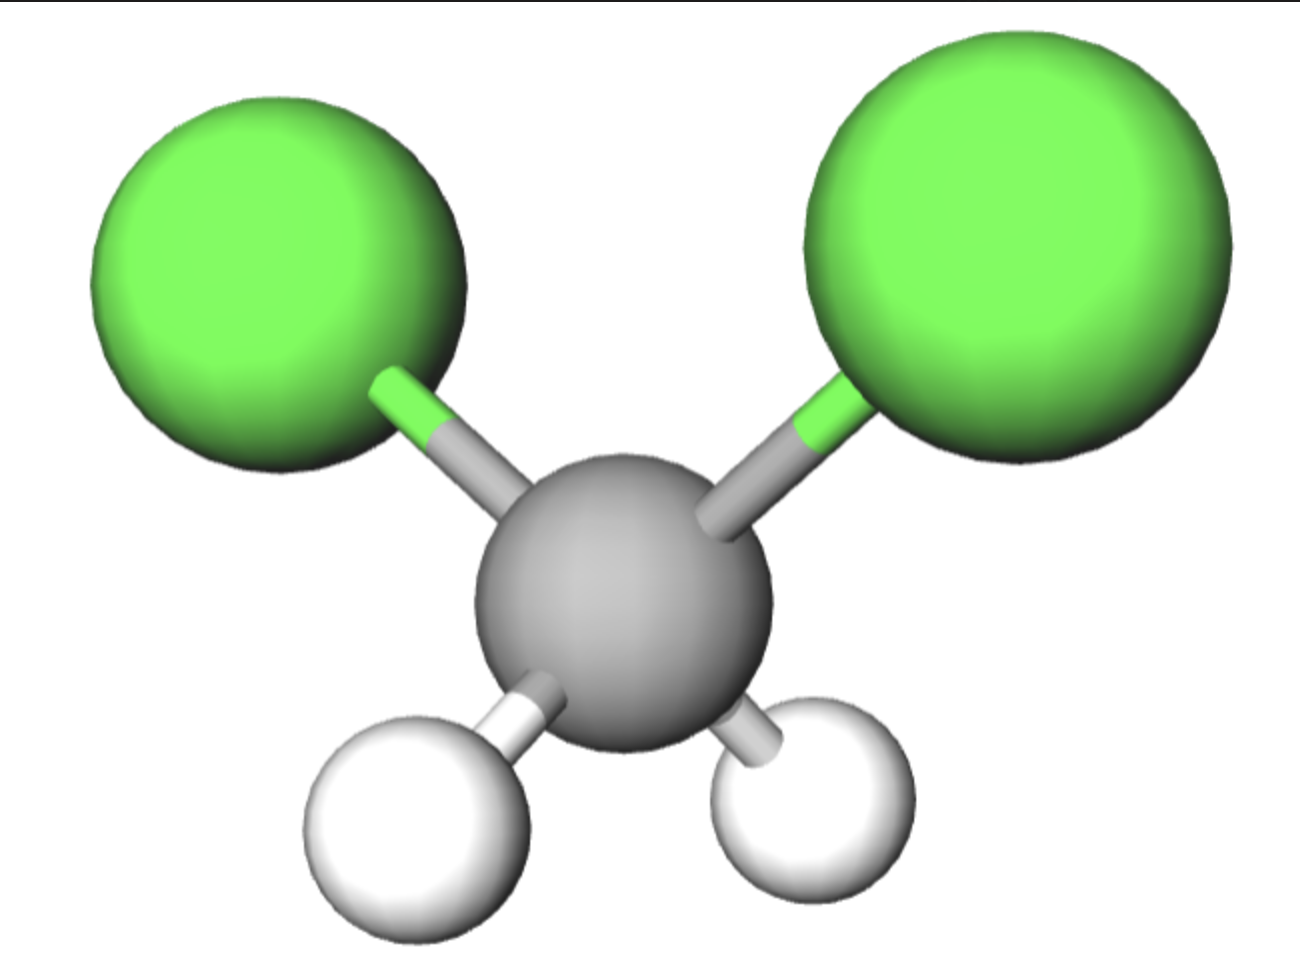
\includegraphics[width=0.4\textwidth]{images/raman_spectra/dcm_i.png}
    \caption{Dichloromethane, ball and stick model. Green: chlorine; gray: carbon; white: hydrogen}
    \label{fig:dcm_i}
\end{wrapfigure}


    Figures \ref{fig:dcm_x} and \ref{fig:dcm_l} show experimental and literature spectra of dichloromethane, CH\(_2\)Cl\(_2\), which is one carbon atom with two covalent bonds to hydrogen atoms and two to chloride atoms, see Figure \ref{fig:dcm_i}. This 5-atomic molecule has 3*5-6, so 9 vibrational modes, all of which are raman active. Table \ref{table:dcm} compares the recorded peaks to literature values, as well as notes the assigned vibrational modes. 

    \begin{table}[h]
    \begin{center}
        \vspace{10pt}
        \begin{tabular}{|c|c|c|}
         \hline
         Exp. Wavelength (\( cm^{-1} \) ) & Lit. Wavelength  (\( cm^{-1} \) ) & Assingment  \\ 
         \hline
         175 & - & - \\
         295 & 282 & CCl\(_2\) bending \\ 
         714 & 713 & CCl symmetric stretching\\
         750 & 748 & CCl asymmetric stretching\\
         - & 893 & CH\(_2\) rocking \\
         1167 & 1153 & CH\(_2\) twisting\\
         - & 1255 & CH\(_2\) wagging\\
         1434 & 1467 & CH\(_2\)  scissoring\\
         2999 & 2996 & CH symmetric stretching \\
         3067 & 3019 & CH asymmetric stretcing \\
         \hline
        \end{tabular}
        \caption{Comparison of experimental and literature \cite{dcml} values, as well as assingment of peaks in a Raman spectrum of dichloromethane by wavenumber. The experimental value represents the maximum of the measured peak }
        \label{table:dcm}
        \vspace{-15pt}
    \end{center}
    \end{table}

    Table \ref{table:dcm} shows that the measured values match the literature values. The missing peaks at 893 and 1255 \( cm^{-1}\) could be explained by the fact that they might just be too weak to be mentioned, as the corresponding regions in Figure \ref{fig:dcm_x} show slight elevations. The different peaks in Figure \ref{fig:dcm_x} are more pronounced, which might be the result of better quality equipment, specifically the spectrometer, which is able to differenciate between peaks that are very close together. The without assignment might stem from rotational frequencies and not vibrational frequencies.

    \bigskip

    The small peaks with a negative raman shift were not mentioned in the table, but they are the results of Anti-Stokes scattering.

    \bigskip

    The literature values used in Table \ref{table:dcm} and the Figure \ref{fig:dcm_l} are not the same, so there are some differences, but they are small. Different sources record slightly different values. Figre \ref{fig:dcm_l} is used to demonstrate the relative intensities of the raman bands.

    \begin{figure}[h]
        \centering
        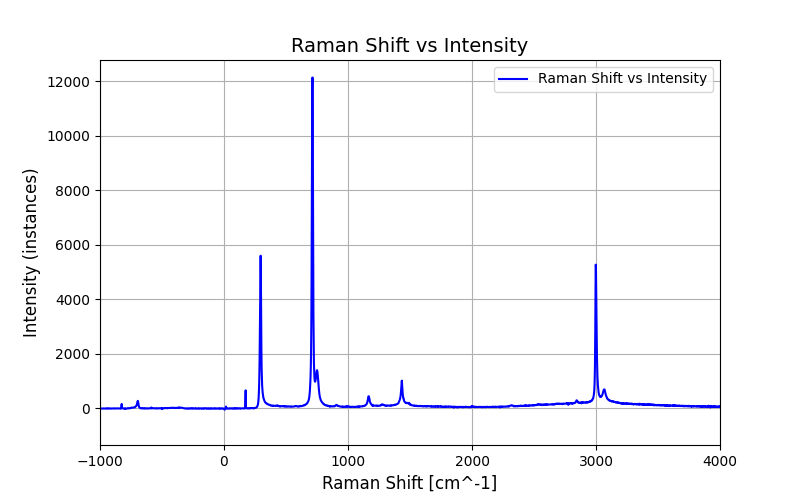
\includegraphics[width=\textwidth]{images/raman_spectra/raman_shift_DCM.png}
        \caption{Experimental Raman spectrum of dichloromethane}
        \label{fig:dcm_x}
        \vspace{30pt}
    \end{figure}

    \begin{figure}[h]
        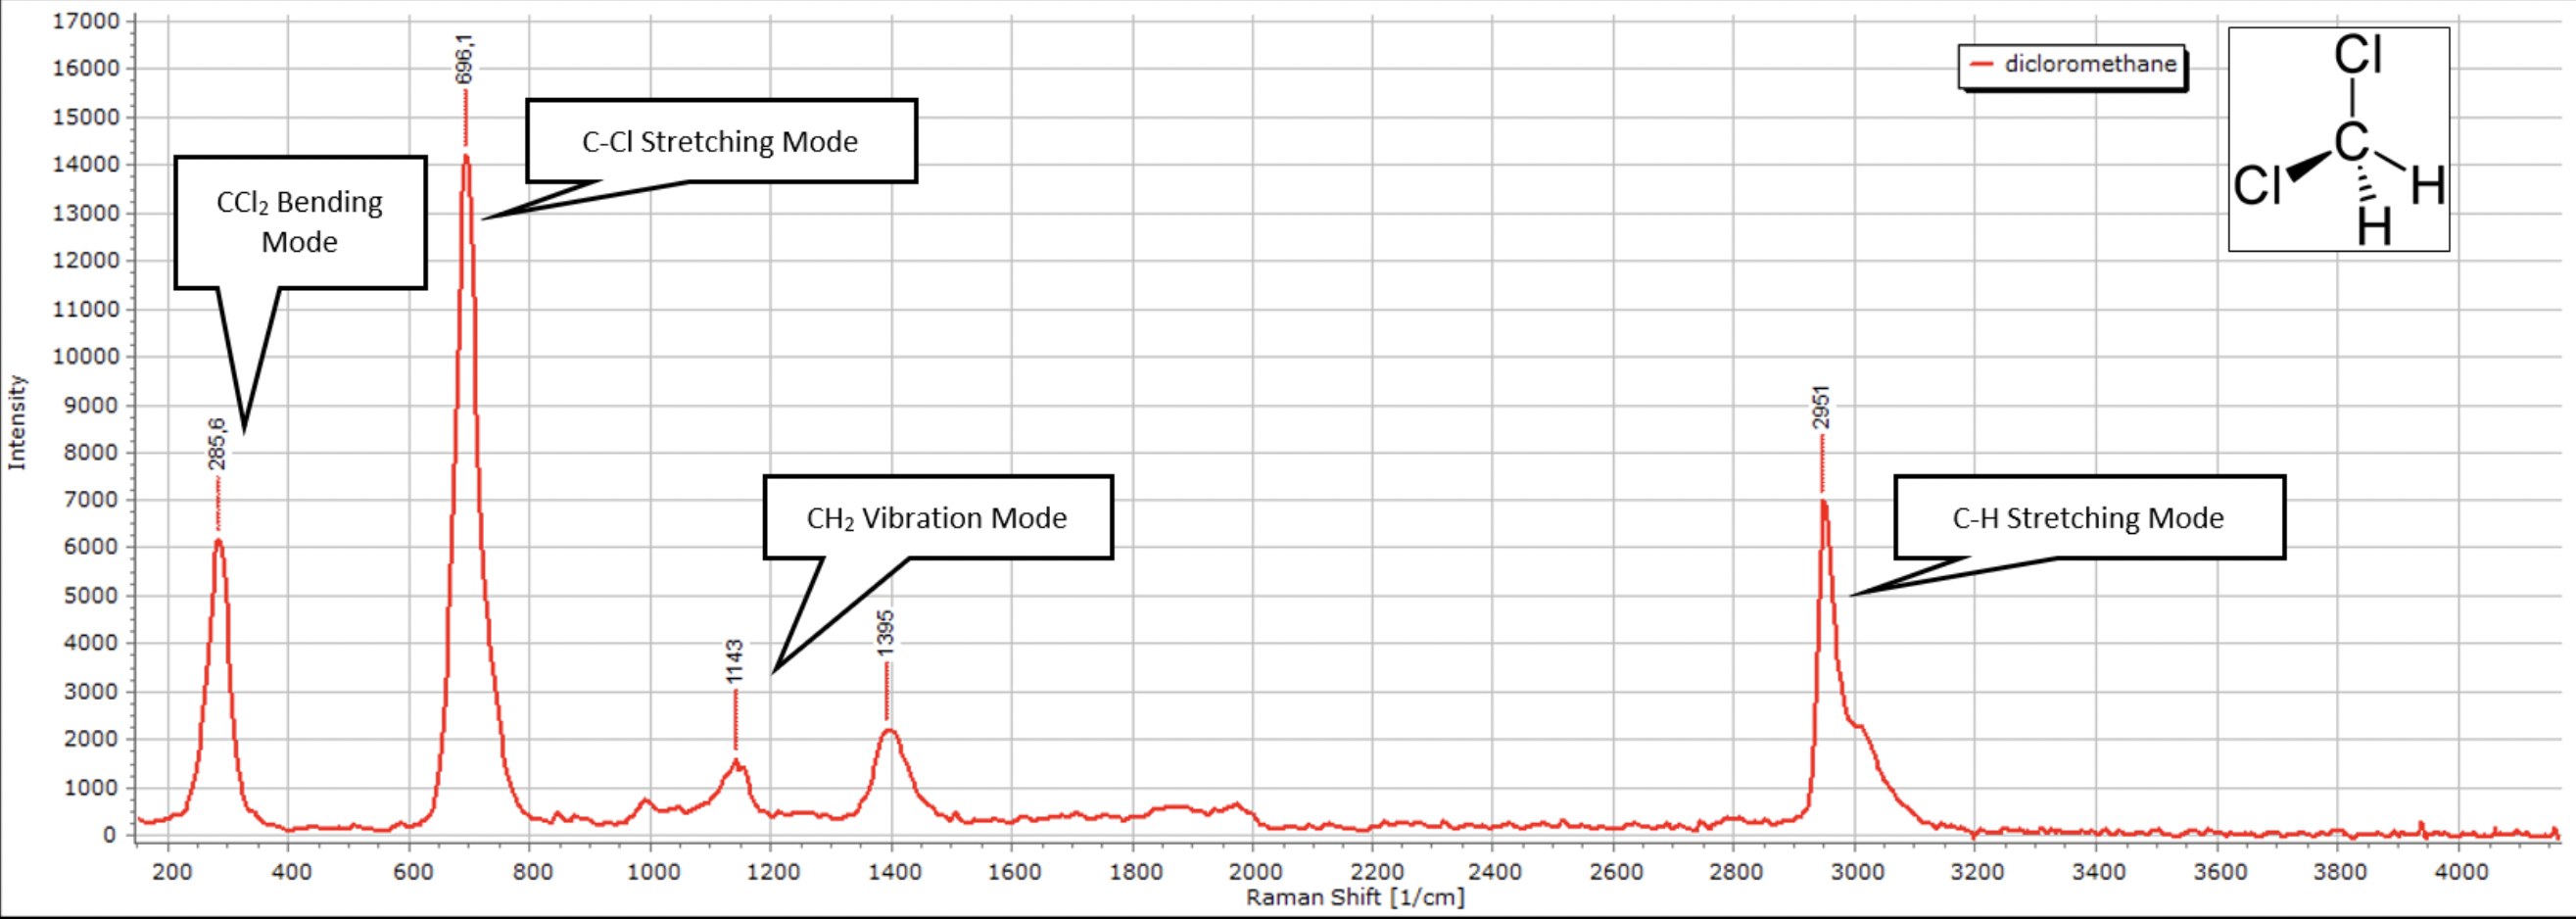
\includegraphics[width=\textwidth]{images/lit_raman/dichloromethane.png}
        \caption{Literature Raman spectrum of dichloromethane \cite{spectrumdcm}}
        \label{fig:dcm_l}
    \end{figure}

    \newpage

\paragraph{Ethanol}

    \begin{wrapfigure}{radiation}{0.5\textwidth} %this figure will be at the right
        \centering
        \vspace{-20pt}
        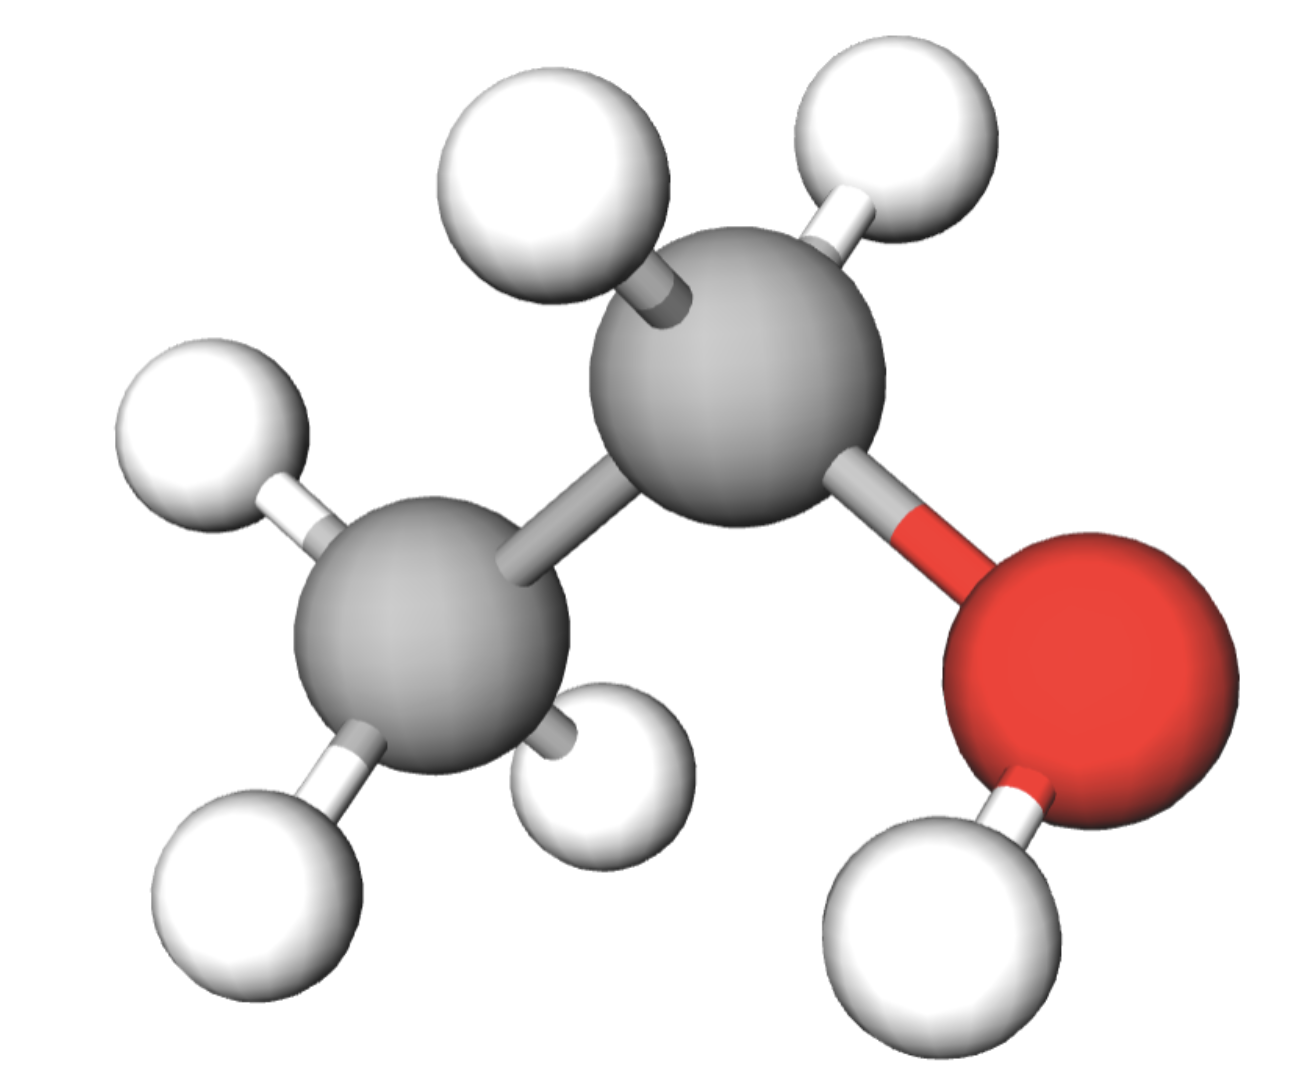
\includegraphics[width=0.4\textwidth]{images/raman_spectra/eth_i.png}
        \caption{Ethanol, ball and stick model. Red: oxygen; gray: carbon; white: hydrogen}
        \label{fig:eth_i}
    \end{wrapfigure}


    Figures \ref{fig:eth_x} and \ref{fig:eth_l} show experimental and literature spectra of ethanol, C\(_2\)H\(_6\)O, see Figure \ref{fig:eth_i}.  Table \ref{table:eth} compares the recorded peaks to literature values, as well as notes the assigned vibrational modes. Raman spectrography can be used to differenciate ethanol from methanol, which is important because while normal alcohol contains ethanol, methanol is toxic to humans.

    \begin{table}[h]
    \begin{center}
        \vspace{15pt}
        \begin{tabular}{|c|c|c|}
         \hline
         Exp. Wavelength (\( cm^{-1} \) ) & Lit. Wavelength  (\( cm^{-1} \) ) & Assingment  \\ 
         \hline
         442 & - & - \\
         894 & 883 & CC stretchung \\ 
         1064 & 1050 & CO stretching\\
         1107 & 1093 & CO stretching\\
         1287 & 1277 & - \\
         1465 & 1454 & CH\(_3\) bending\\
         2891& 2885 &  CH stretching mode\\
         2942 & 2929 & CH stretching mode\\
         2985 & 2974 & CH stretching mode\\
         
         \hline
        \end{tabular}
        \caption{Comparison of experimental and literature \cite{ethl1} \cite{ethl2} values, as well as assingment of peaks in a Raman spectrum of ethanol by wavenumber. The experimental value represents the maximum of the measured peak }
        \label{table:eth}
    \end{center}
    \end{table}

    Table \ref{table:eth} shows that the measured values match the literature values. Sadly, not all bands were assigned and the bands 2891, 2942 and 2985 cm\(^{-1}\) were not differenciated between. Same as with dichloromethane, the peaks are more differenciated in Figure \ref{fig:eth_x} than in the literature Figure \ref{fig:eth_l}. The OH stretching mode was not as clearly identifyable and wasn't recorded for that reason.

    \bigskip
    
    The raman spectrum for methanol wouldn't have the very visible peak at around 900 cm\(^{-1}\) which comes from a CC stretching mode.

    The literature values used in Table \ref{table:eth} and the Figure \ref{fig:eth_l} are not the same, so there are some differences, but they are small. Different sources record slightly different values. 

    

    \newpage

    \begin{figure}[h]
        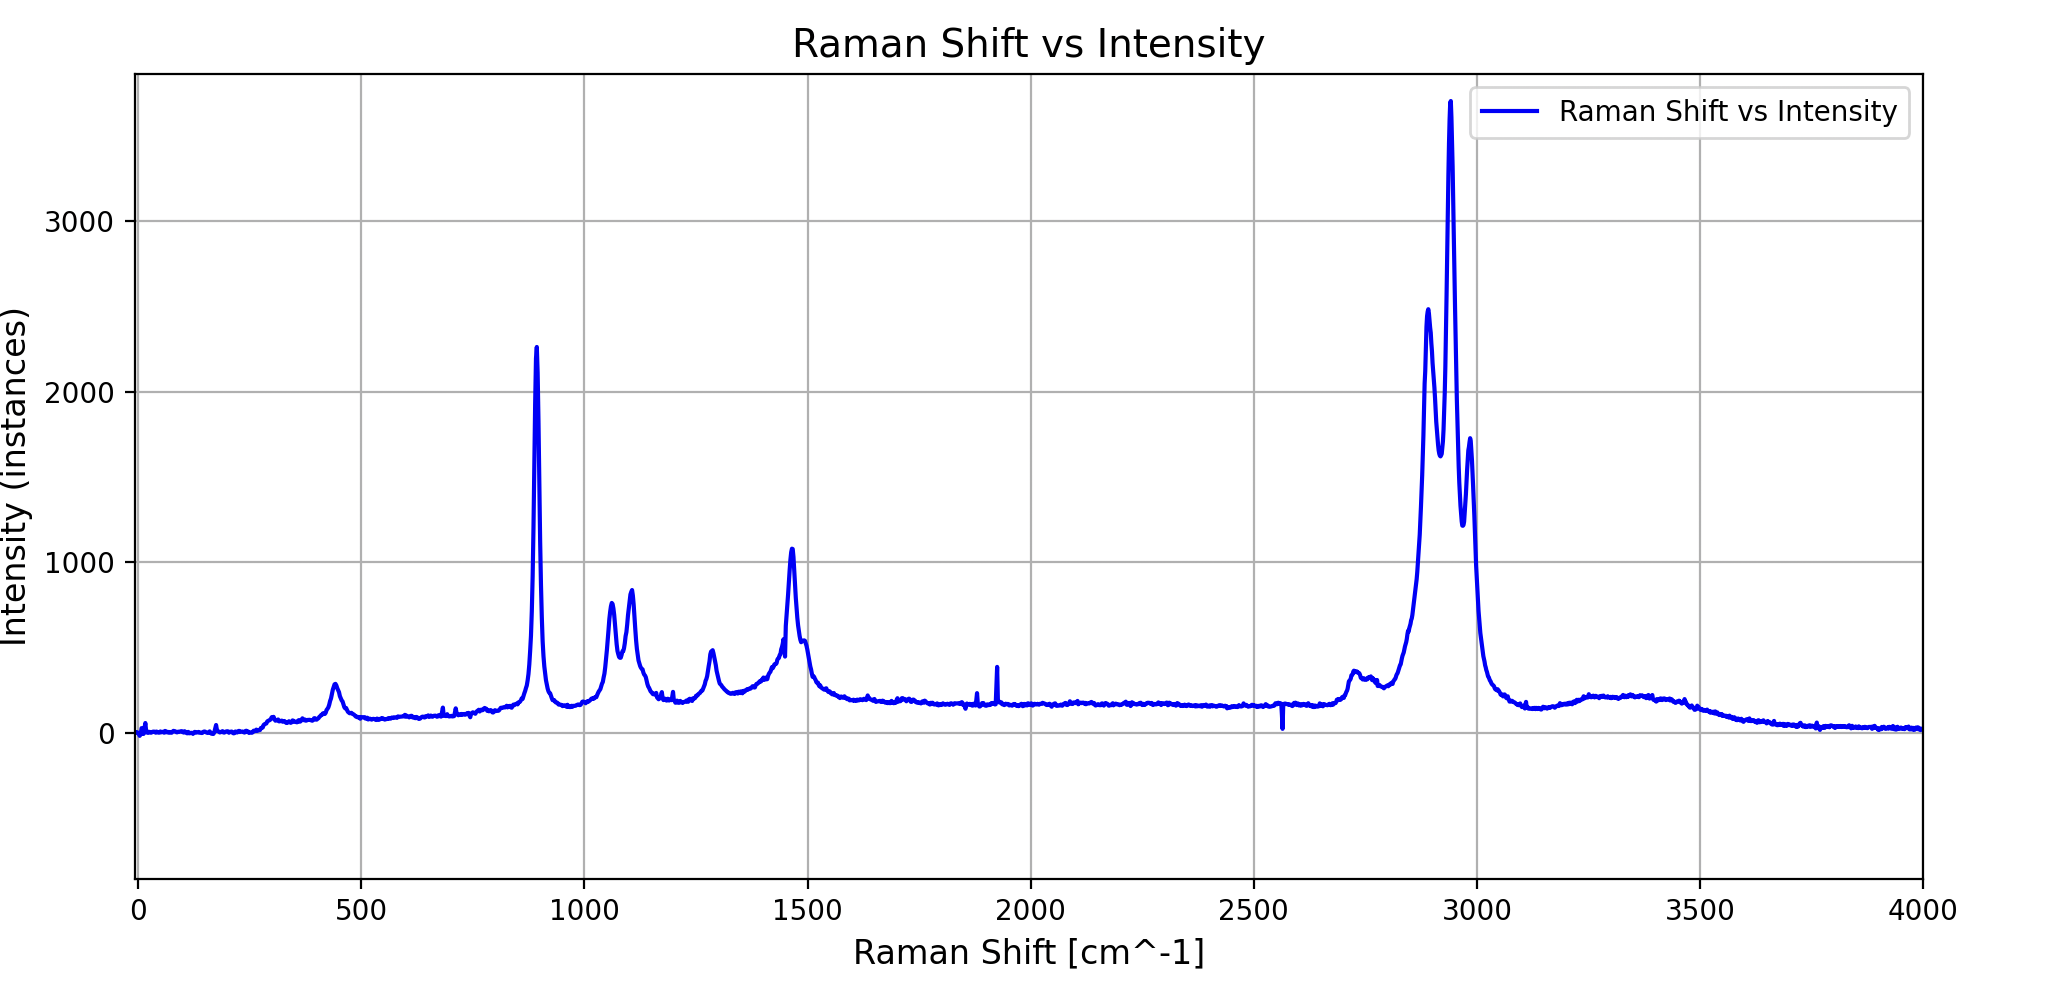
\includegraphics[width=\textwidth]{images/raman_spectra/raman_shift_ethanol.png}
        \caption{Experimental Raman spectrum of ethanol}
        \label{fig:eth_x}
        \vspace{30pt}
    \end{figure}


    \begin{figure}[h]
        \centering
        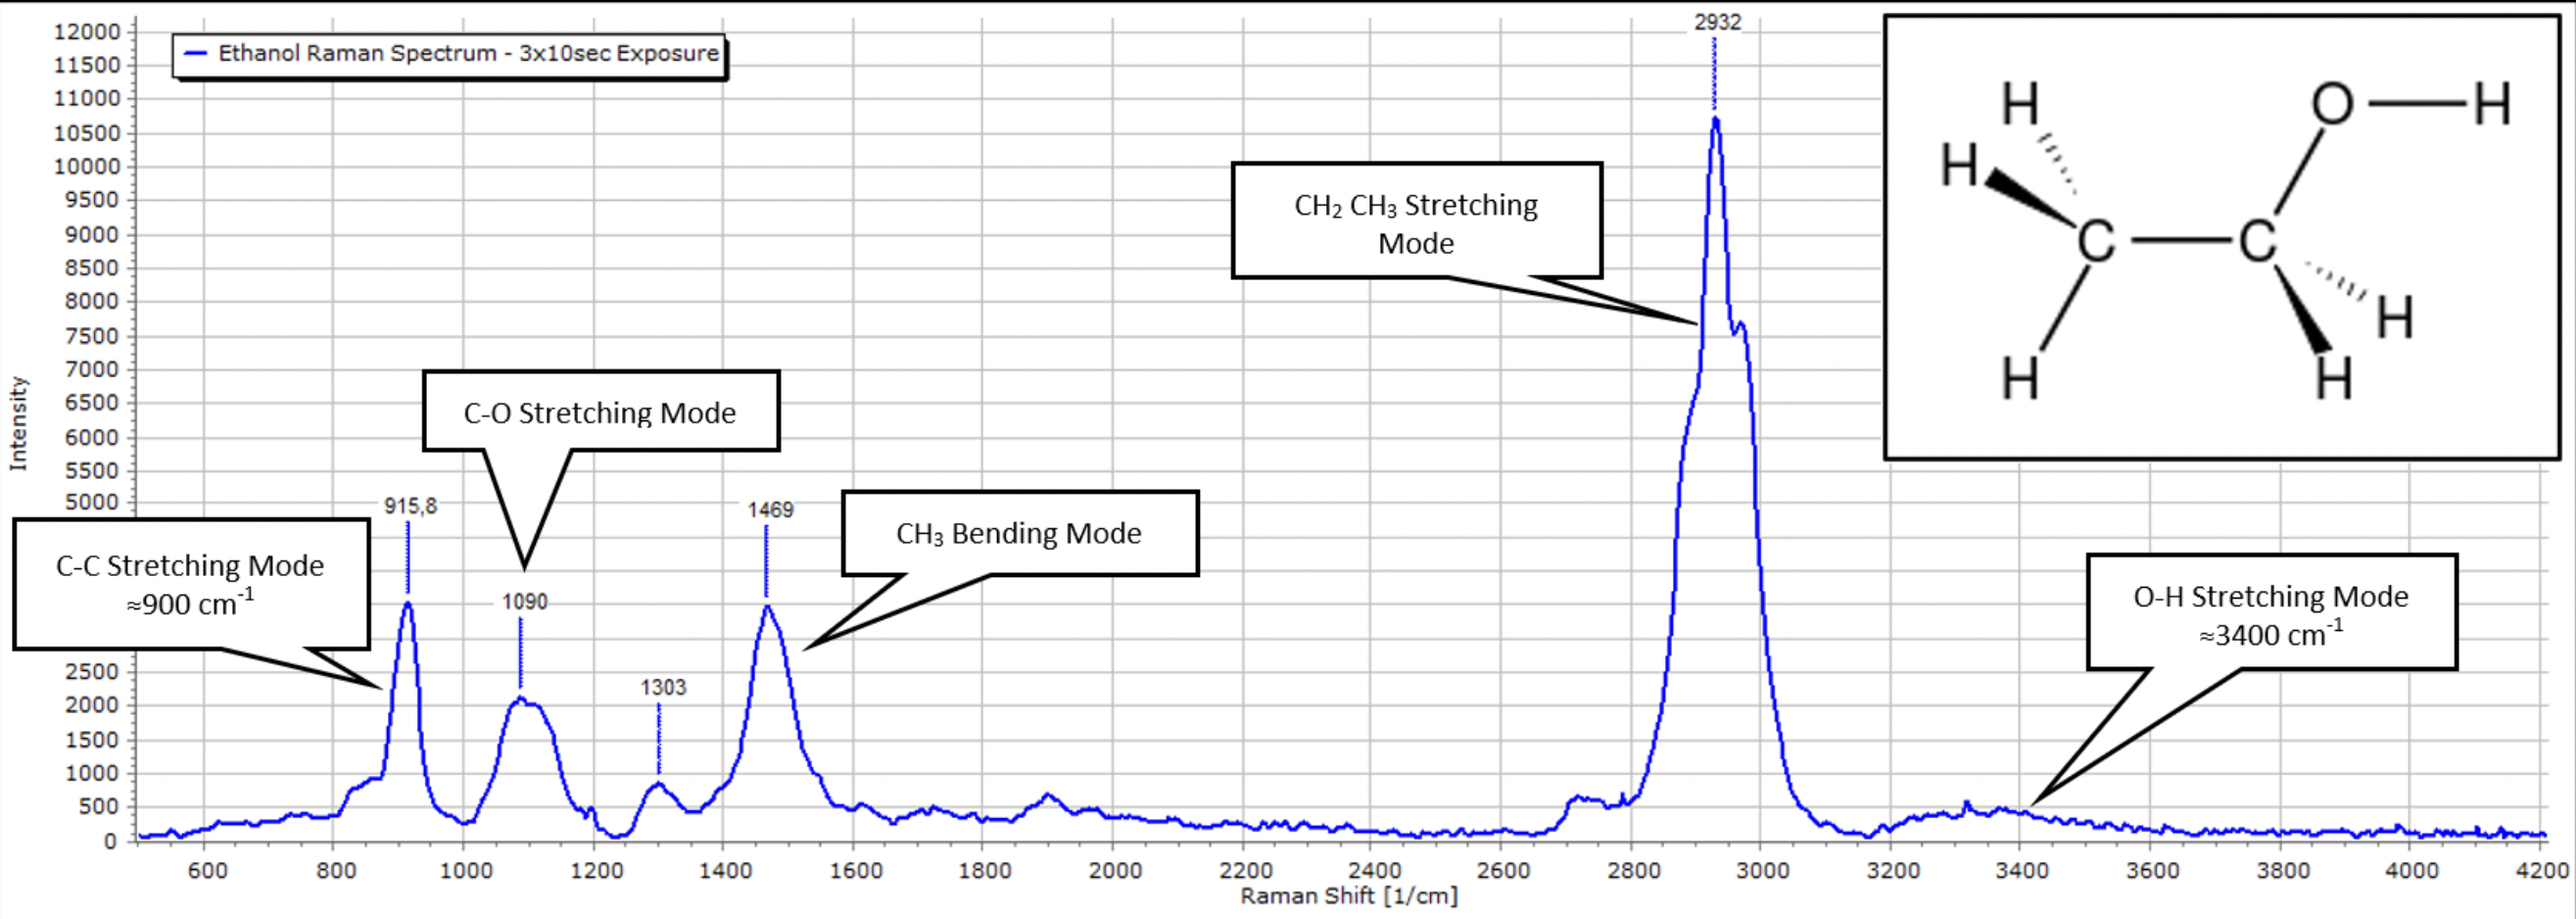
\includegraphics[width=\textwidth]{images/lit_raman/ethanol.png}
        \caption{Literature Raman spectrum of ethanol \cite{spectrumet} }
        \label{fig:eth_l}
    \end{figure}

    \newpage

    \paragraph{Polyethylene (PE)}

    \begin{wrapfigure}{radiation}{0.5\textwidth} %this figure will be at the right
        \centering
        \vspace{-20pt}
        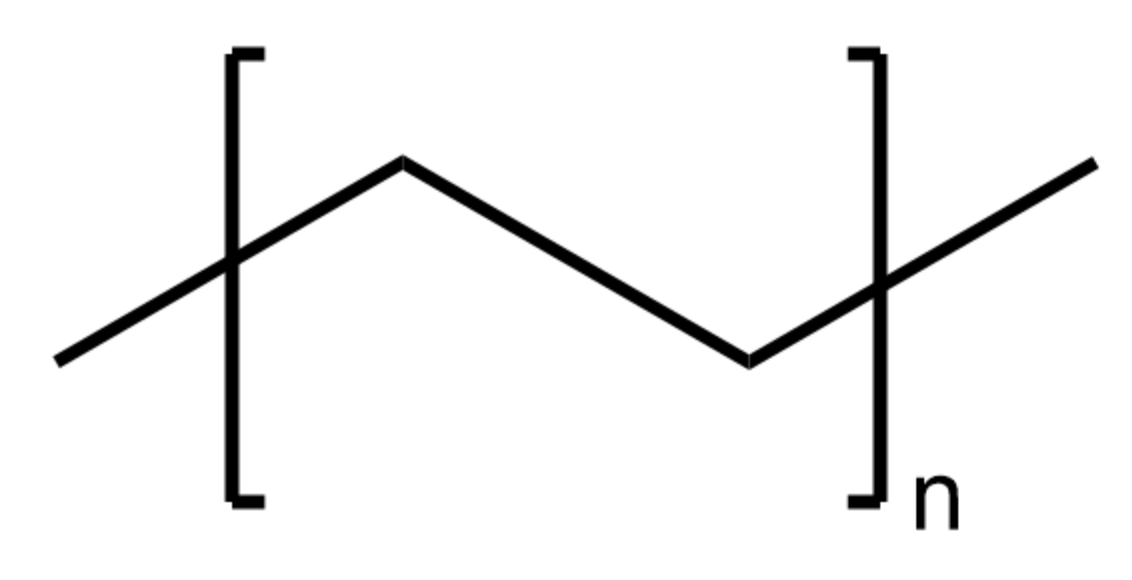
\includegraphics[width=0.4\textwidth]{images/raman_spectra/pe_i.png}
        \caption{Polyethylene, skeleton model}
        \label{fig:pe_i}
    \end{wrapfigure}


    Figures \ref{fig:pe_x} and \ref{fig:pe_l} show experimental and literature spectra of polyethylene, (C\(_2\)H\(_2\))\(_n\), see Figure \ref{fig:pe_i}. \\
    The same unit, C\(_2\)H\(_2\), is repeated an undefined amount of times, which results in a long carbon chain Table \ref{table:eth} compares the recorded peaks to literature values, as well as notes the assigned vibrational modes. 

    \begin{table}[h]
    \begin{center}
        \vspace{15pt}
        \begin{tabular}{|c|c|c|}
         \hline
         Exp. Wavelength (\( cm^{-1} \) ) & Lit. Wavelength  (\( cm^{-1} \) ) & Assingment  \\ 
         \hline
         0 & - & reflections laser light \\
         175 & - & - \\
         1072 & 1062 & CC stretching crystalline\\ 
         1091 & 1079 & CC stretching amorphous\\
         1139 & 1128 & CC stretching\\
         1180 & 1169 & CH\(_2\) rocking\\
         1305 & 1294 & CH\(_2\) twisting\\
         1379 & 1369 & CH\(_3\) wagging amorphous\\
         1428 & 1416 & CH\(_2\) bending \\
         1451 & 1439 & CH\(_2\) bending\\
         1468 & 1462 & CH\(_2\) bending\\
         2861& 2848 &  CH\(_2\) symmetric stretching\\
         2892& 2882 &  CH\(_2\) asymmetric stretching\\
         \hline
        \end{tabular}
        \caption{Comparison of experimental and literature \cite{pel1} \cite{pel2} values, as well as assingment of peaks in a Raman spectrum of polyethylene by wavenumber. The experimental value represents the maximum of the measured peak }
        \label{table:pe}
    \end{center}
    \end{table}

    Table \ref{table:pe} shows that the measured values match the literature values. Since PE is semicrystalline, some values, for example at 1379 cm\(^{-1}\) and 1091 cm\(^{-1}\) correspond to vibrational modes in amorphous regions, some in crystalline, and some, like 1468 cm\(^{-1}\), are influenced by both. Peaks that are exclusive to crystalline structures, like the one at 1428 cm\(^{-1}\), can be used to evaluate the degree of crystallinity.

    \bigskip
    
    The literature values used in Table \ref{table:pe} and the Figure \ref{fig:pe_l} are not the same, so there are some differences, but they are small. Different sources record slightly different values. For PE, often only the peaks between 1000 cm\(^{-1}\) and 1600 cm\(^{-1}\) are looked at, which is the reason for the multiple sources in Table \ref{table:pe}.

    

    \newpage

    \begin{figure}[h]
        \centering
        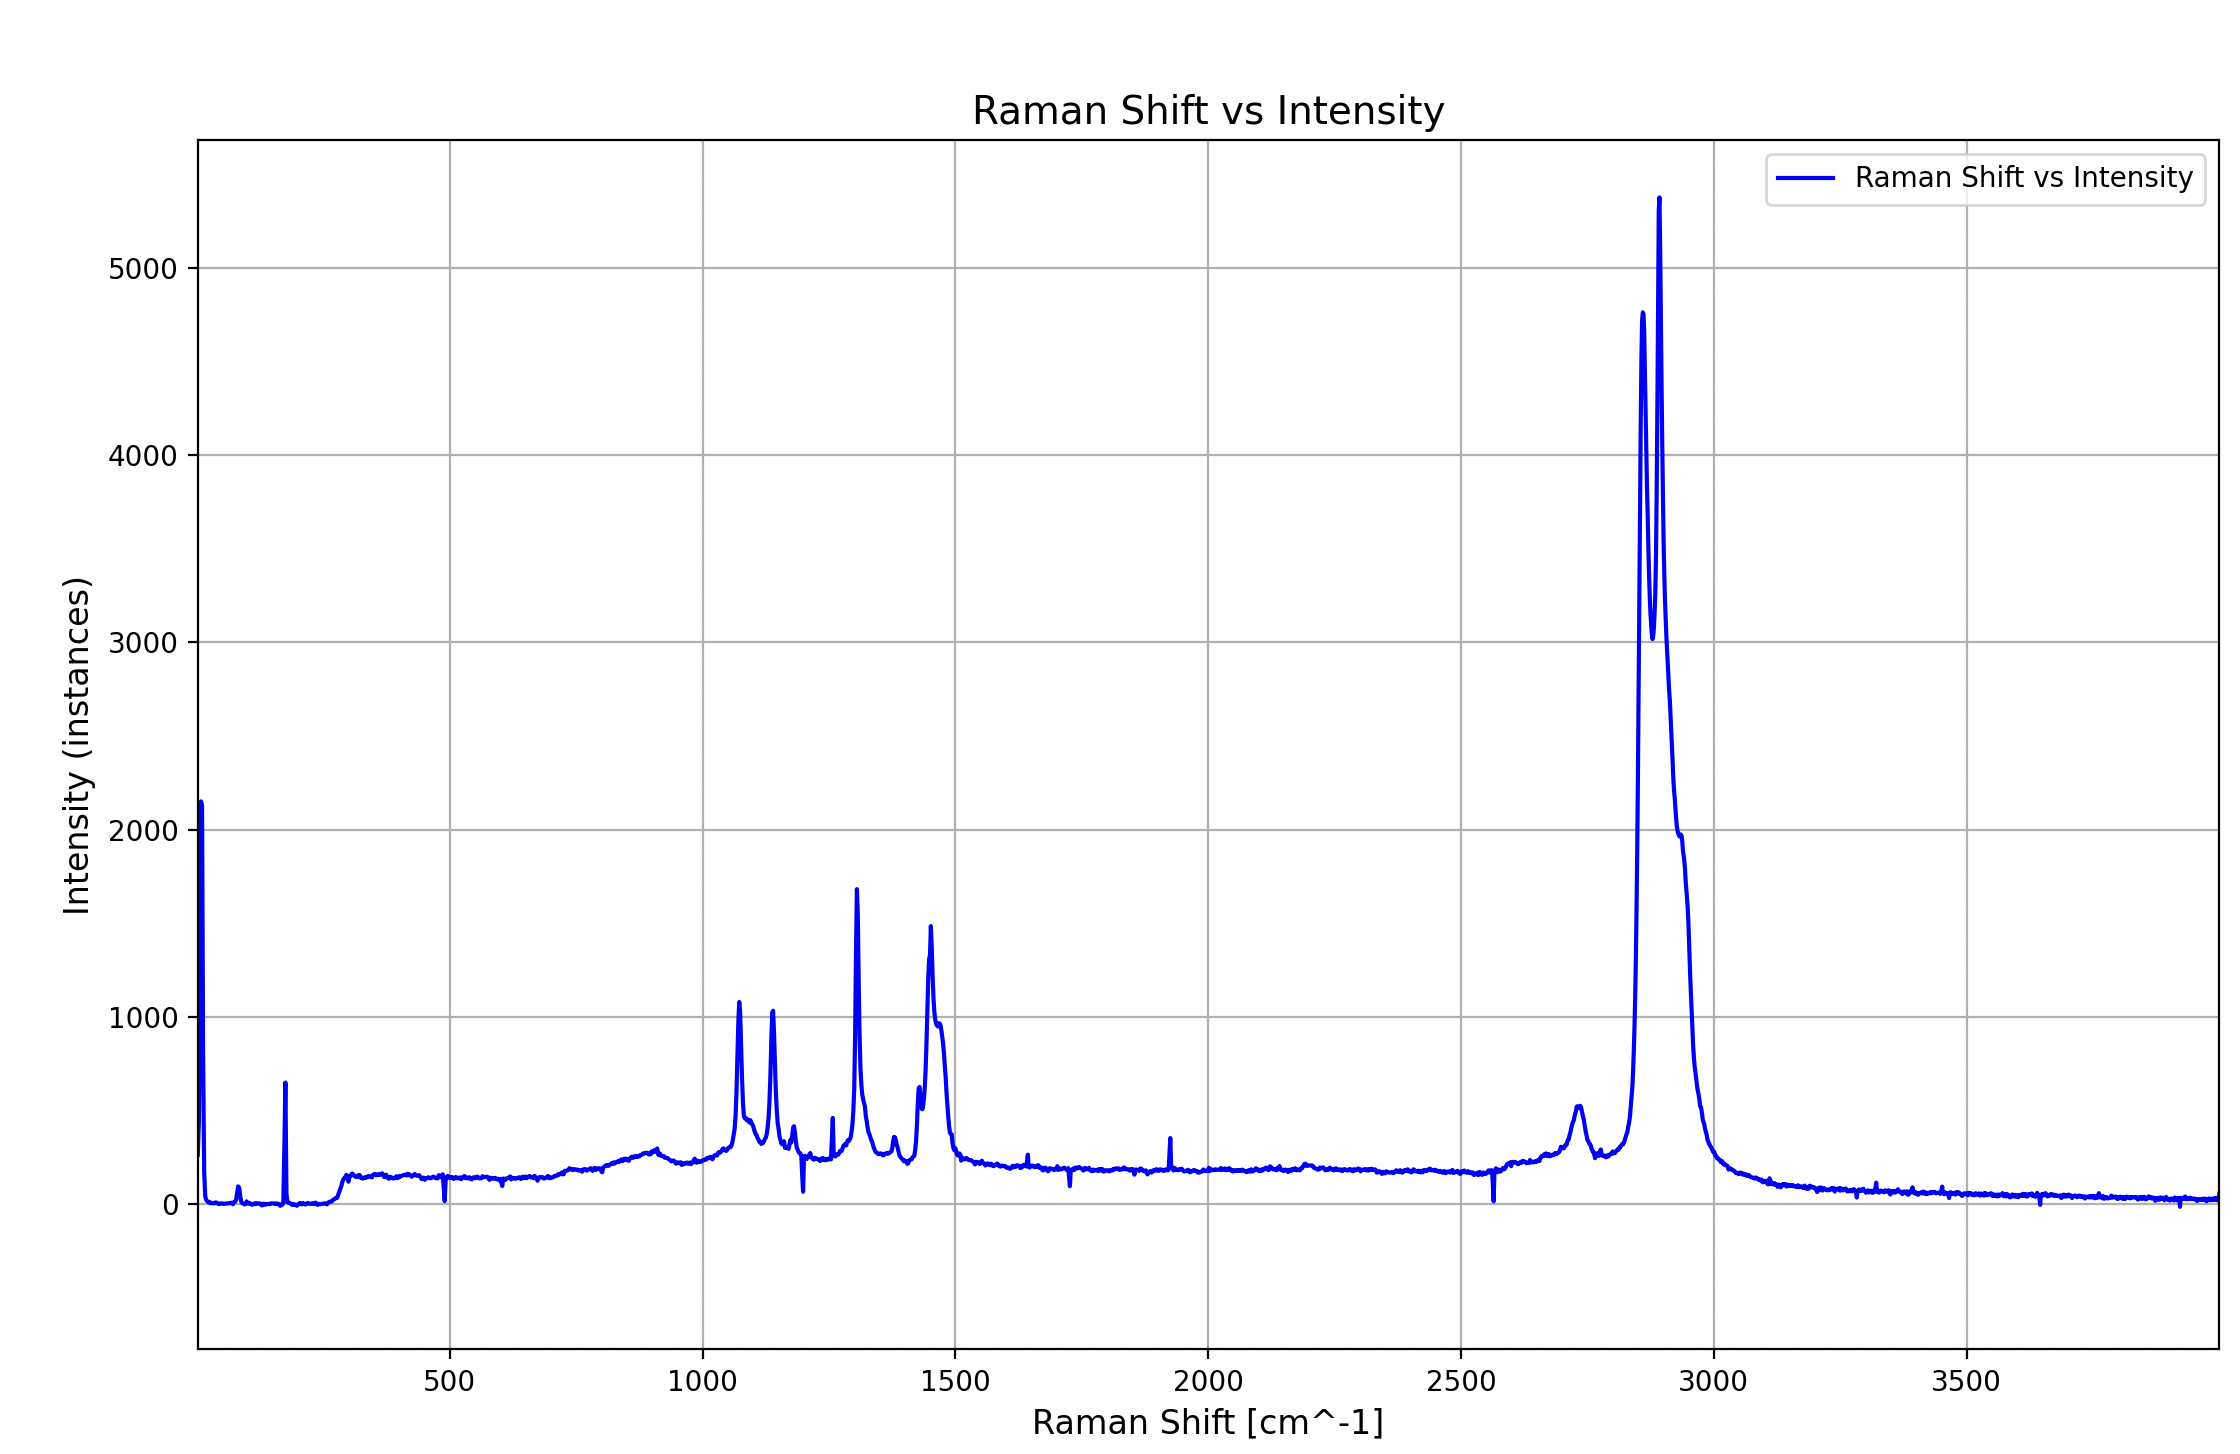
\includegraphics[width=\textwidth]{images/raman_spectra/raman_shift_polyethyleneh.png}
        \caption{Experimental Raman spectrum of polyethylene}
        \label{fig:pe_x}
    \end{figure}

    \begin{figure}[h]
        \centering
        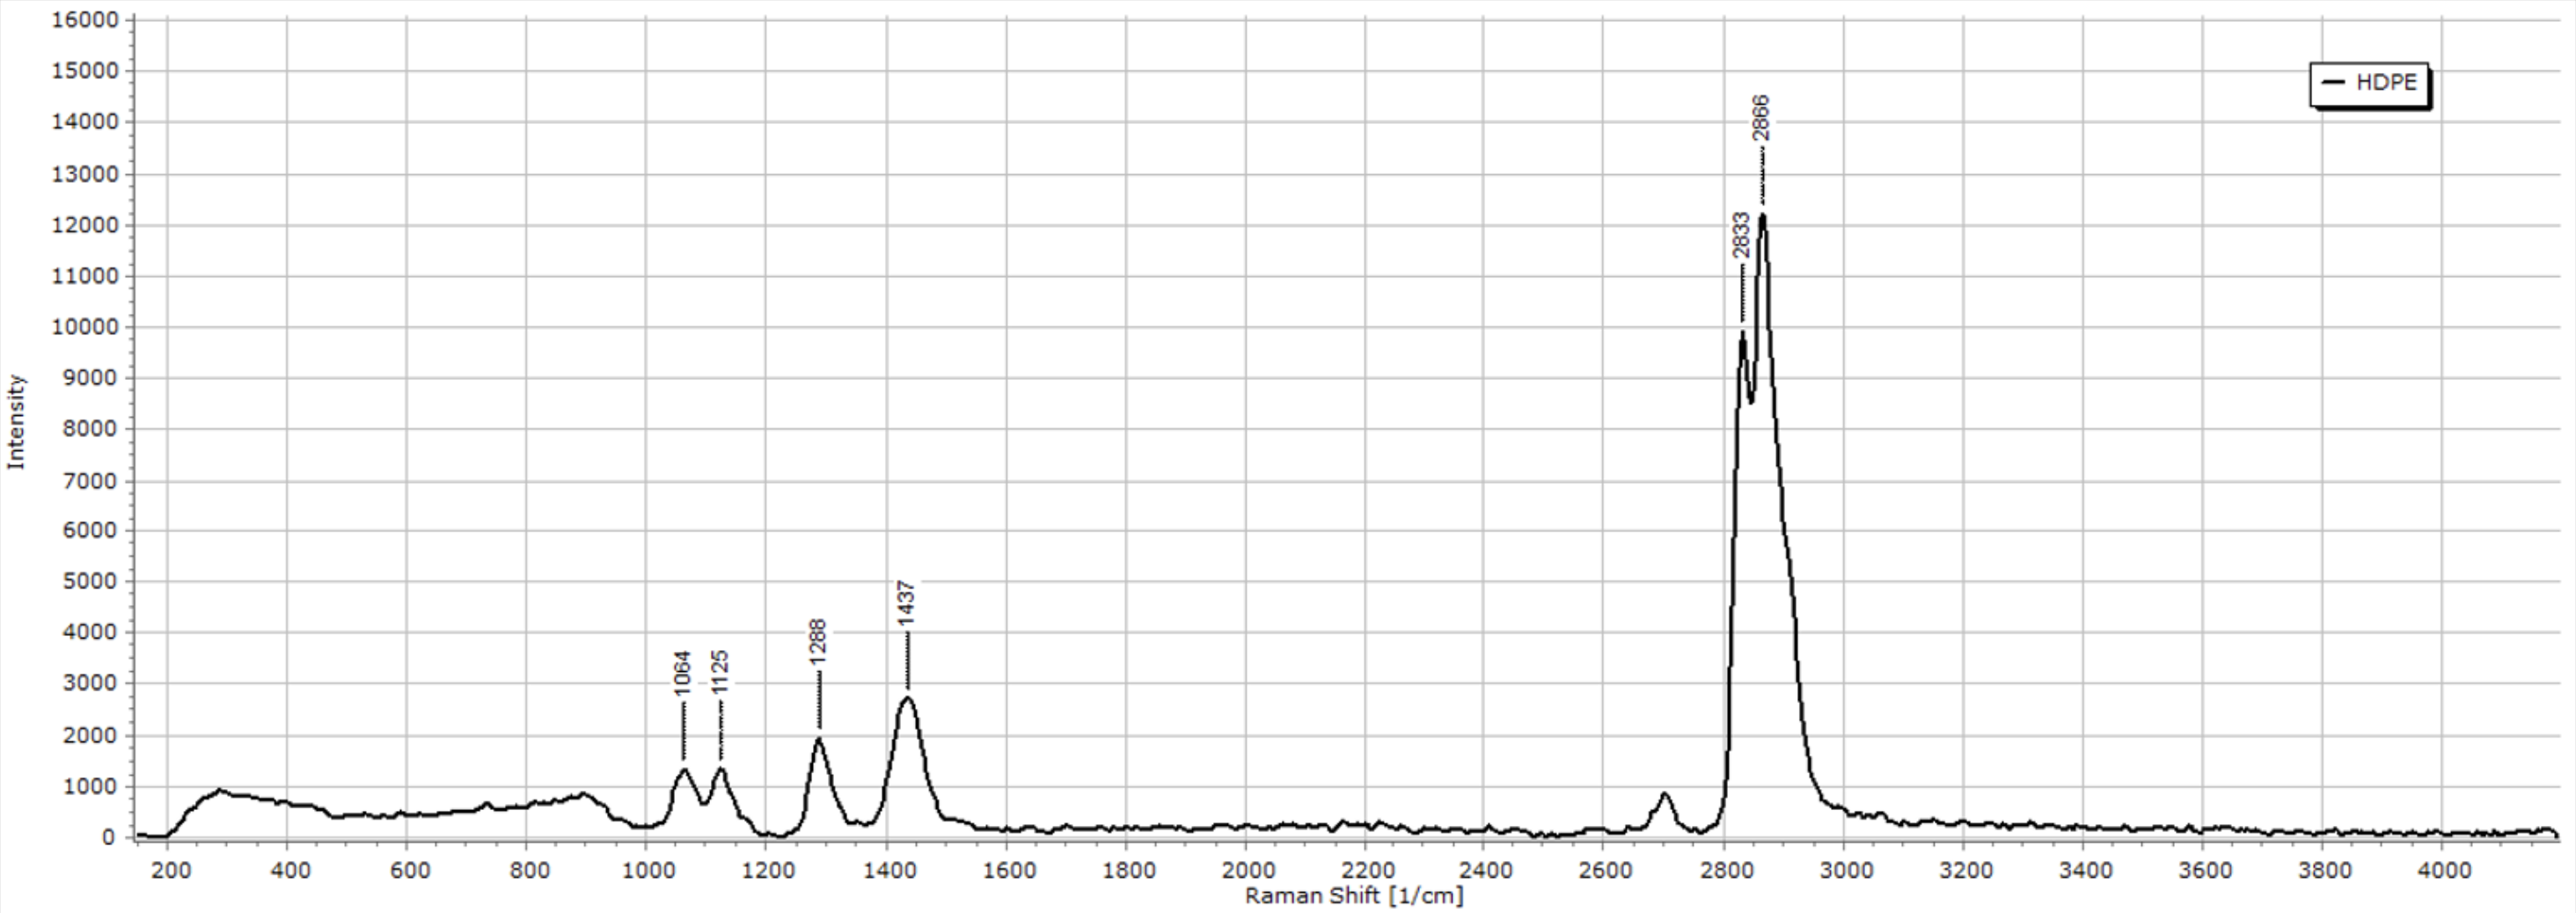
\includegraphics[width=\textwidth]{images/lit_raman/HDPE.png}
        \caption{Literature Raman spectrum of polyethylene \cite{spectrap}}
        \label{fig:pe_l}
    \end{figure}

    \newpage

    \paragraph{Polystyrene (PS)}
    
    \begin{wrapfigure}{radiation}{0.4\textwidth} %this figure will be at the right
        \centering
        \vspace{-20pt}
        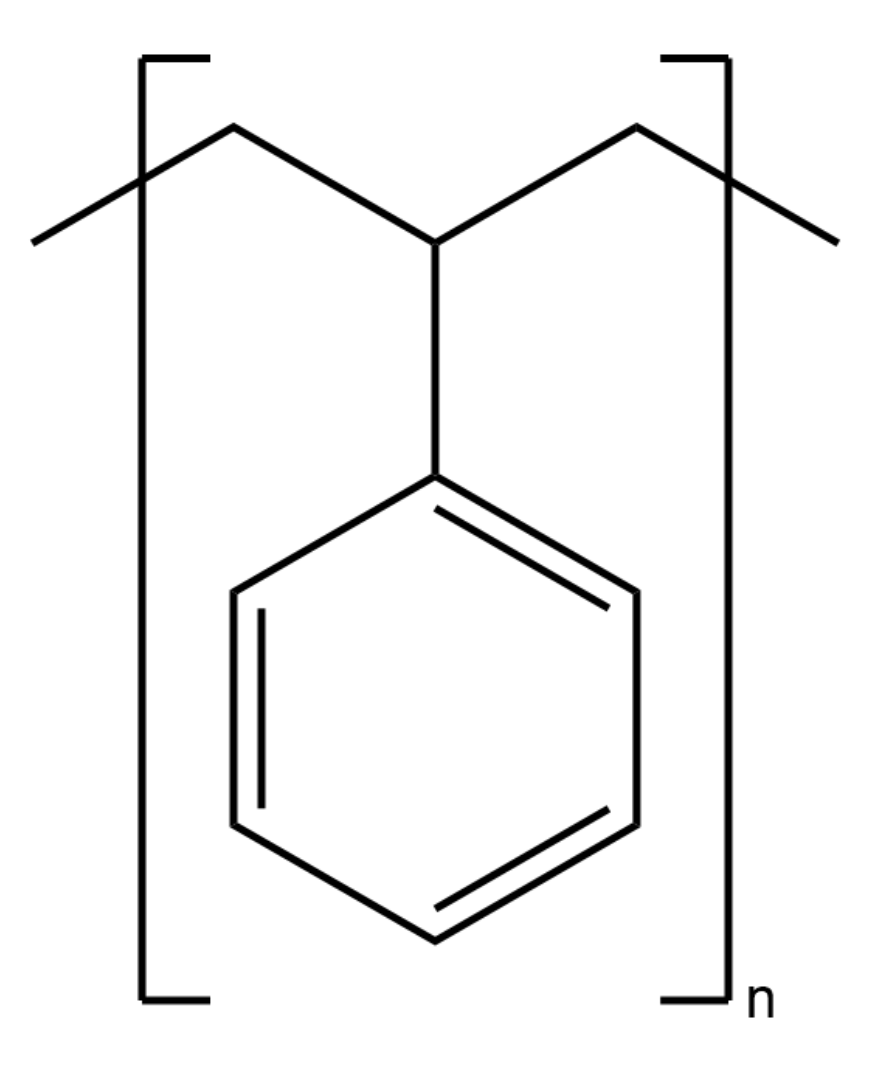
\includegraphics[width=0.3\textwidth]{images/raman_spectra/ps_i.png}
        \caption{Polystyene, skeleton model}
        \label{fig:ps_i}
    \end{wrapfigure}


    Figures \ref{fig:ps_x} and \ref{fig:ps_l} show experimental and literature spectra of polystyrene, (C\(_8\)H\(_8\))\(_n\) see Figure \ref{fig:pe_i}.\\ 
    The unit C\(_8\)H\(_8\), a benzene ring attached to an ethane chain and repeated an undefined number of times, results in a carbon chain with every second carbon atom being attached to a benzene ring. Table \ref{table:eth} compares the recorded peaks to literature values, as well as notes the assigned vibrational modes. 

    \begin{table}[h]
    \begin{center}
        \vspace{15pt}
        \begin{tabular}{|c|c|c|}
         \hline
         Exp. Wavelength (\( cm^{-1} \) ) & Lit. Wavelength  (\( cm^{-1} \) ) & Assingment  \\ 
         \hline
         631 & 621 & ring deformation mode \\
         805 & 795 & CH out-of-plane deformation \\
         1012 & 1001 & ring breathing mode\\ 
         1041 & 1031 & CH in-plane deformation \\
         1165 & 1155 & C-C stretching\\
         1461 & 1450 & H\(_2\) scissoring\\
         1594 & 1583 & C=C stretch\\
         1613 & 1602 & ring-skeletal stretch\\
         2923 & 2915 & CH\(_2\) antisymmetric stretch\\
         3068 & 3060 & CH aromatic stretch  \\
         \hline
        \end{tabular}
        \caption{Comparison of experimental and literature \cite{ps1} \cite{ps2} values, as well as assingment of peaks in a Raman spectrum of polyethylene by wavenumber. The experimental value represents the maximum of the measured peak }
        \label{table:ps}
    \end{center}
    \end{table}

    Table \ref{table:pe} shows that the measured values match the literature values. A greater degree of precision could be achieved by averaging more scans or using longer exposure times, as well as ensuring the absence of any other light during the recording of the spectra.

    \bigskip
    
    The literature values used in Table \ref{table:ps} and the Figure \ref{fig:ps_l} are not the same, so there are some differences, but they are small. Different sources record slightly different values. Often only the peaks up to 2000 cm\(^{-1} \) are considered, which is the reason for the multiple sources in Table \ref{table:ps}. 
    

    \newpage

    \begin{figure}[h]
        \centering
        \makebox[\textwidth][c]{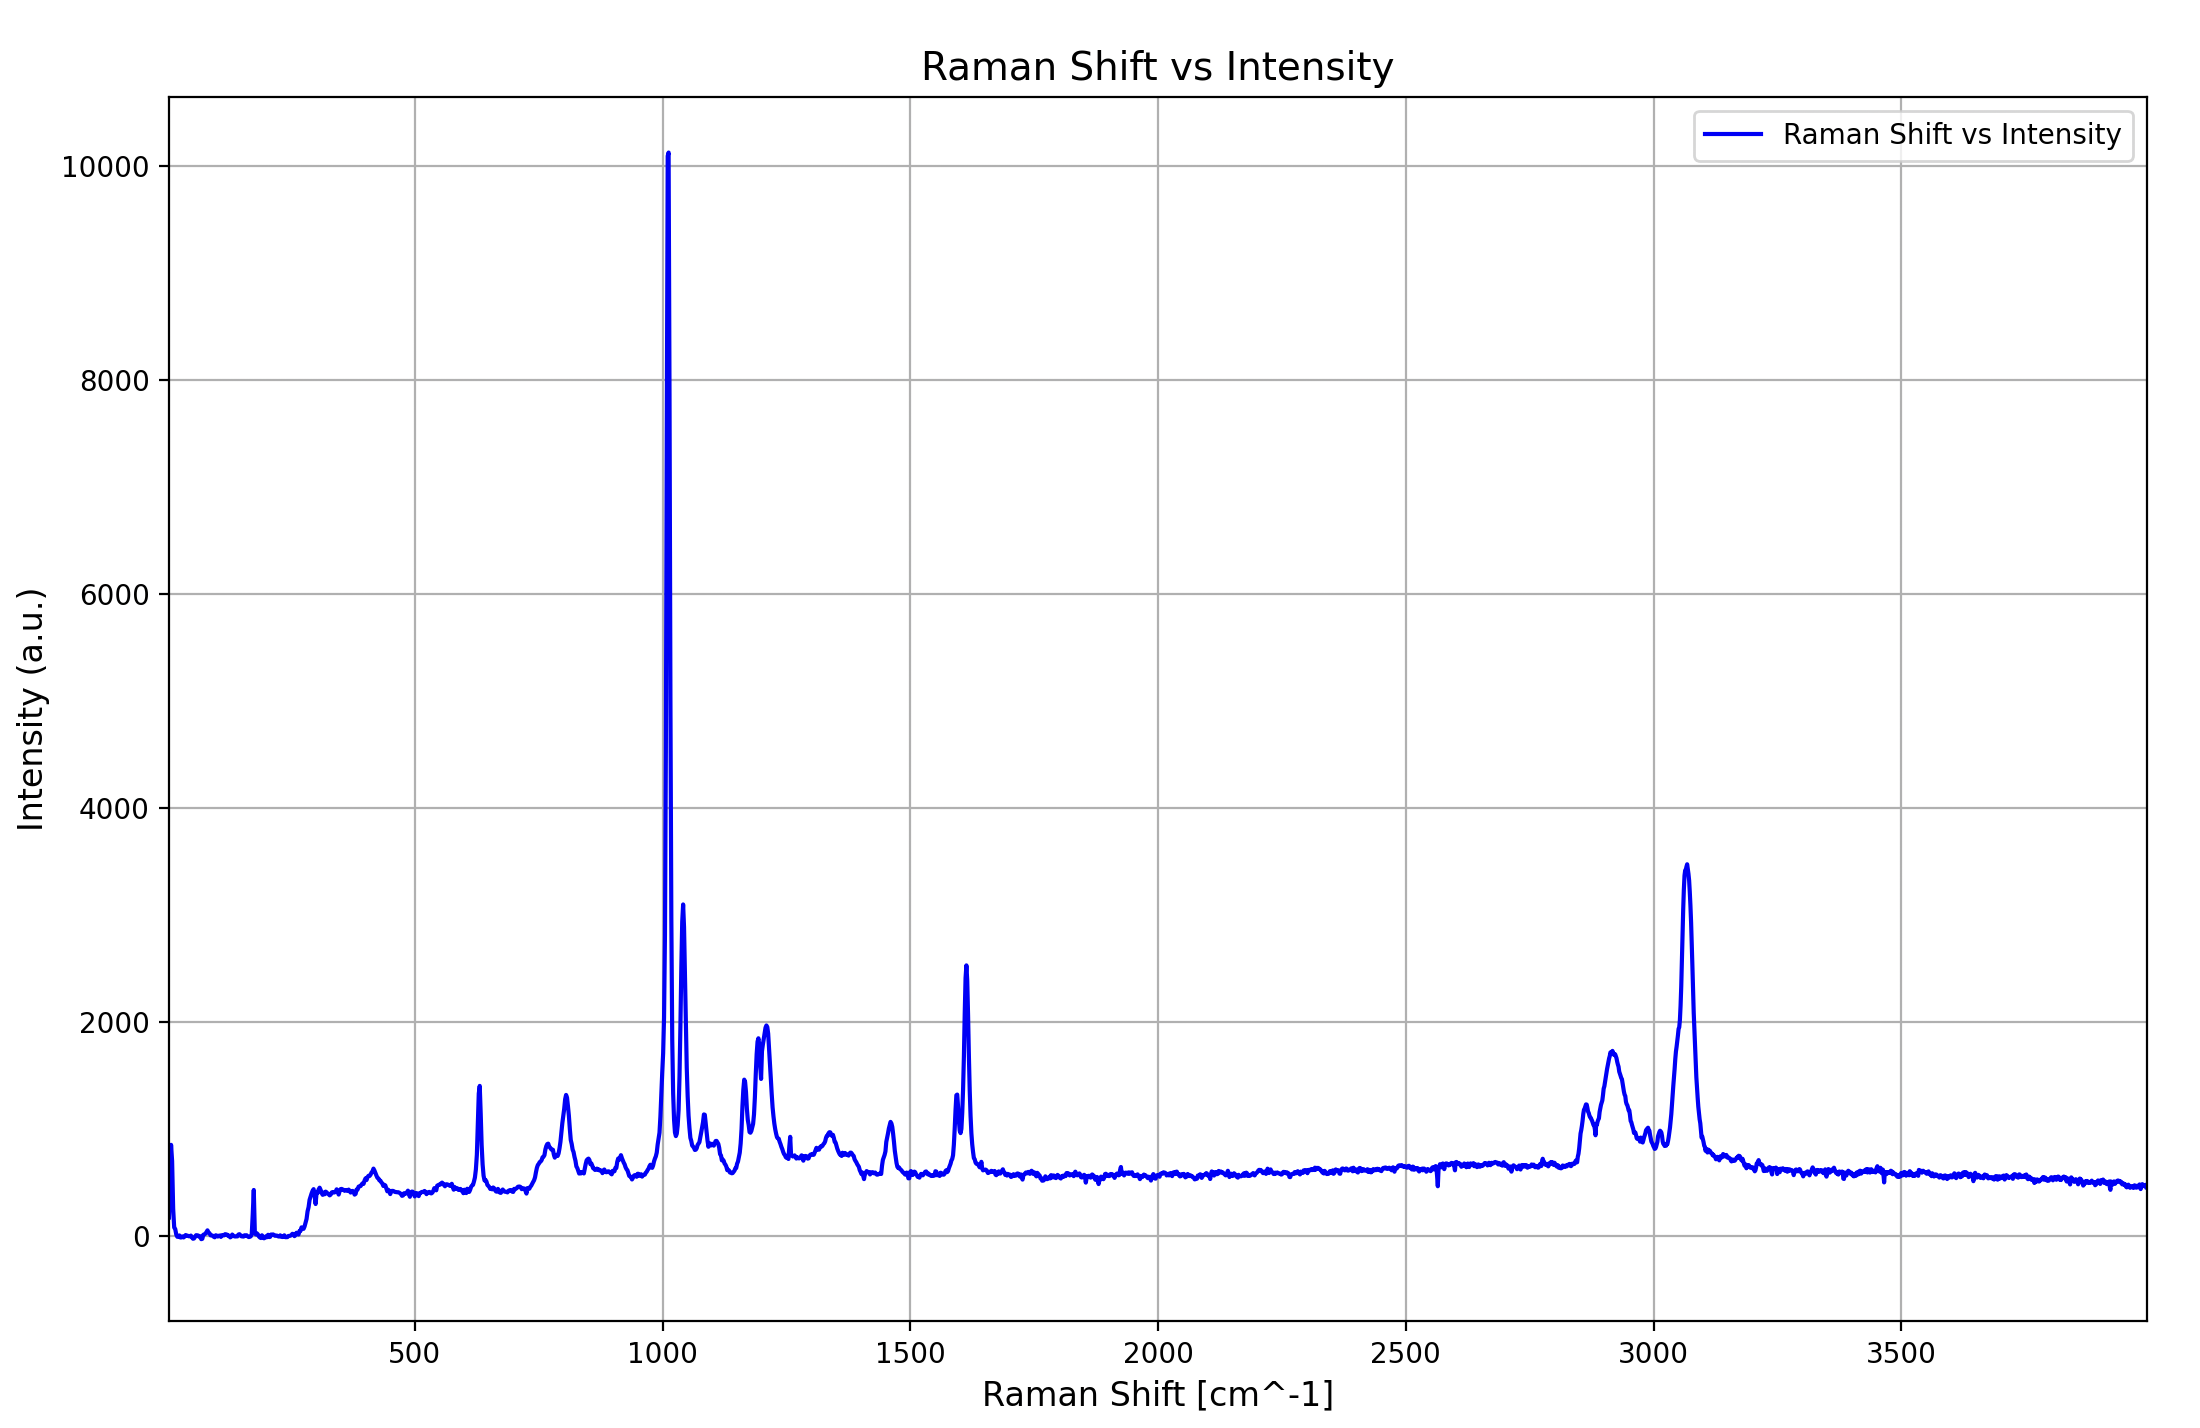
\includegraphics[width=1.2\textwidth]{images/raman_spectra/raman_shift_polystyreneh.png}}
        \caption{Experimental Raman spectrum of polystyrene}
        \label{fig:ps_x}
    \end{figure}

    \begin{figure}[h]
        \centering
        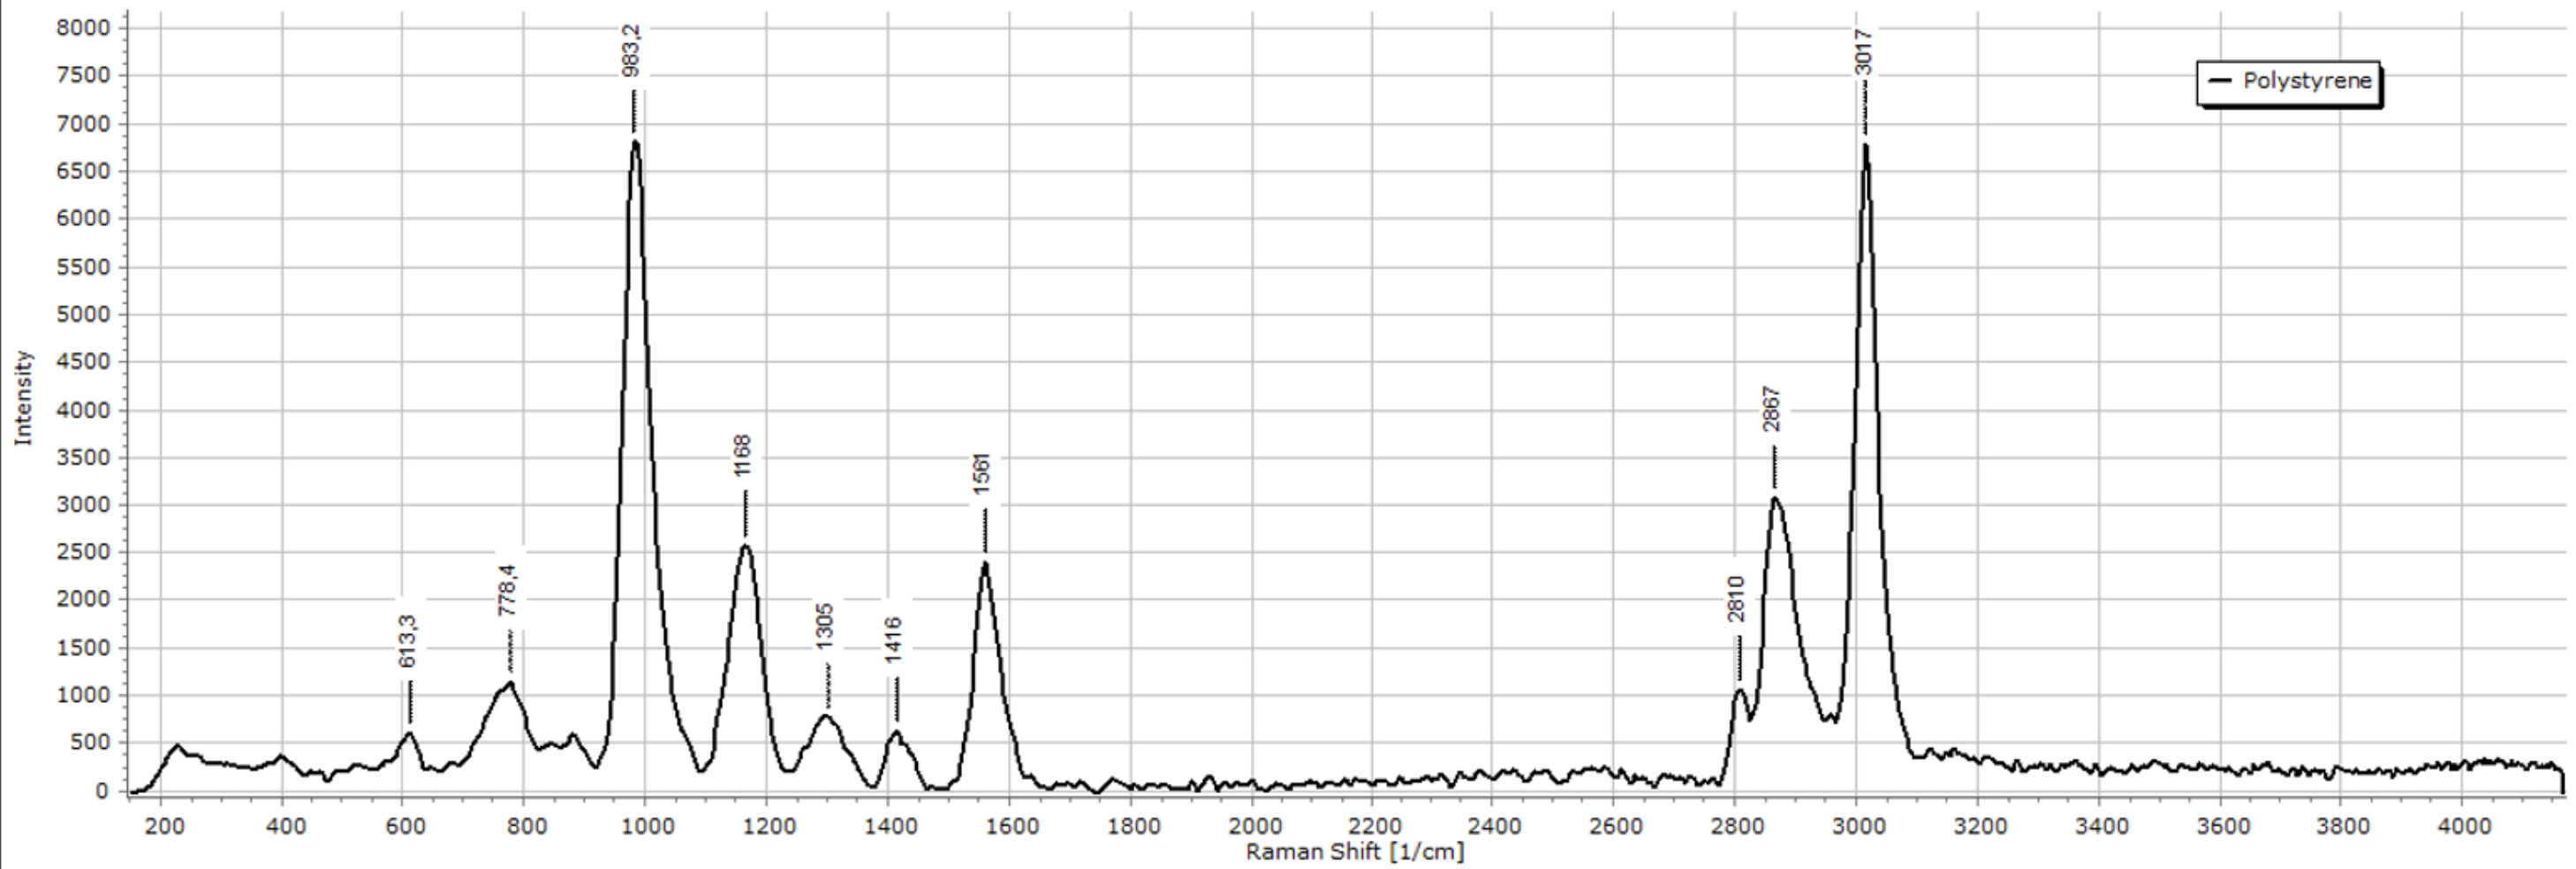
\includegraphics[width=\textwidth]{images/lit_raman/PS.png}
        \caption{Literature Raman spectrum of polystyrene \cite{spectrap}}
        \label{fig:ps_l}
    \end{figure}
